\section{Experimental Evaluation}
\subsection{Geometric validity and generation cost}
We executed six fixed base requests under three conditions: full Composer,
the same request with the protected union disabled, and a restricted generator
with oval sections, no branches/chambers and no geometric modifiers. Four
requests are normal cases; two are declared intrusion/roughness stress cases.
All 18 attempts use a 0.35\,m sphere plus 0.20\,m margin, visual/collision
voxel sizes 0.24/0.32\,m, a four-million-voxel ceiling and a 300\,s invocation
budget. There are no replacement seeds or generation retries. Explicit layouts
do not invoke stochastic layout screening, so this is not a screening ablation.

The initial delivery importer retained OBJ texture-seam vertices and rejected
the visual boundary as non-watertight. We declared an importer amendment,
merged only exactly coincident positions and rechecked the same immutable
triangles. Table~\ref{tab:generator} reports these corrected outcomes; the
original rejections remain archived. All three conditions accept 4/4 normal
requests. On the two stress requests, Composer accepts 1/2, no protection 0/2,
and restricted 2/2. One stress request produces a large disconnected void
component under both full and unprotected generation and is rejected. The
other unprotected request has endpoints outside the conservative robot grid.
Thus protection helps one retained stress case, while the restricted geometry
has higher overall yield in this pilot. Six purposively fixed requests are
insufficient for a statistical advantage or robustness claim.
Figures~\ref{fig:pilot} and~\ref{fig:protection} show the aggregate outcomes
and the retained protection diagnostic, respectively.

Seventeen fixed transverse planes per delivered mesh measure enclosing
section span, area, nonconvexity and centroid-direction proxies. These
measurements include junctions and chambers: they expose the difference between
nominal construction dimensions and actual geometry, rather than demonstrate
accurate diameter tracking. Full normal outputs retain the requested branch
and chamber cases and nonuniform sections; the restricted outputs omit these
mechanisms. No exact free-space branch/loop count or real-cave distribution
match is established. Wall-clock costs include failed attempts, both import
checks and measurements on a shared workstation, not isolated throughput.
Figure~\ref{fig:cases} separates geometric appearance from texture changes.

A separate analytic fixture suite detects four injected faults: a thin slab,
a local cap, a visual-only slab and a post-export width contraction below the
robot diameter. Both analytically clear controls pass. Labels follow explicit
box/slab inequalities, not checker outputs. This six-fixture diagnostic is not
an estimate of arbitrary-mesh detector accuracy. Disabling generation protection
changes geometry; bypassing this checker would instead change acceptance.

Actual PLUME native and supported graph-input smoke runs were attempted on
a pinned upstream revision. Native execution was blocked by the Windows
\texttt{noise} build dependency; graph input reached upstream mesh generation
but failed at an incompatible Blender 5.2 geometry-node API. No comparable
PLUME yield or timing is reported, and unsupported settings are not counted
as algorithmic failures.
\begin{table}[t]
\centering
\caption{Descriptive generation pilot, after declared OBJ seam recheck. Costs include failed attempts and both delivery checks. PLUME comparison was blocked.}
\label{tab:generator}
\small
\begin{tabular}{lccc}
\toprule
Condition & Normal & Stress & s / accepted \\
\midrule
Composer & 4/4 & 1/2 & 11.12 \\
No protection & 4/4 & 0/2 & 12.72 \\
Restricted & 4/4 & 2/2 & 4.76 \\
PLUME & \missing & \missing & \missing \\
\bottomrule
\end{tabular}
\end{table}

\begin{figure*}[t]
\centering
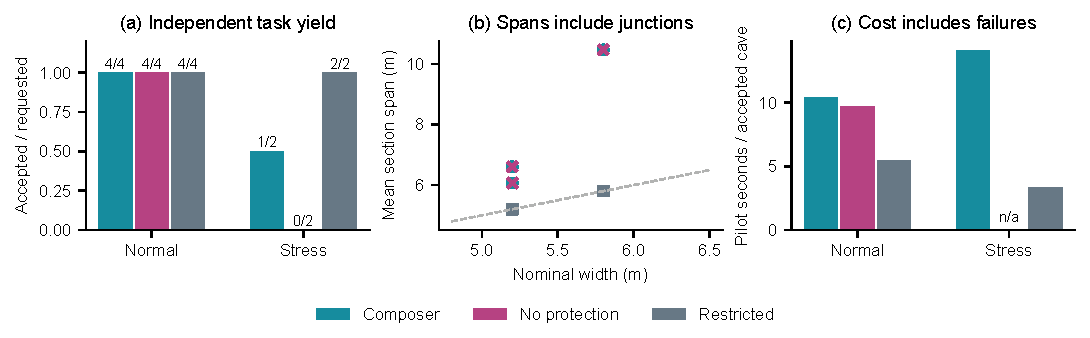
\includegraphics[width=\textwidth]{figures/generated/c1_v02/pilot_quantitative.pdf}
\caption{Descriptive generation pilot after the declared exact-position OBJ seam
recheck: six base requests, eighteen single attempts. Section spans include
junctions and chambers and are not precise diameter-control errors. Cost
includes failed attempts and measurement; no-protection stress cost per
accepted cave is undefined because neither request passed. No policy or PLUME
comparison is represented.}
\label{fig:pilot}
\end{figure*}
\begin{figure*}[t]
\centering
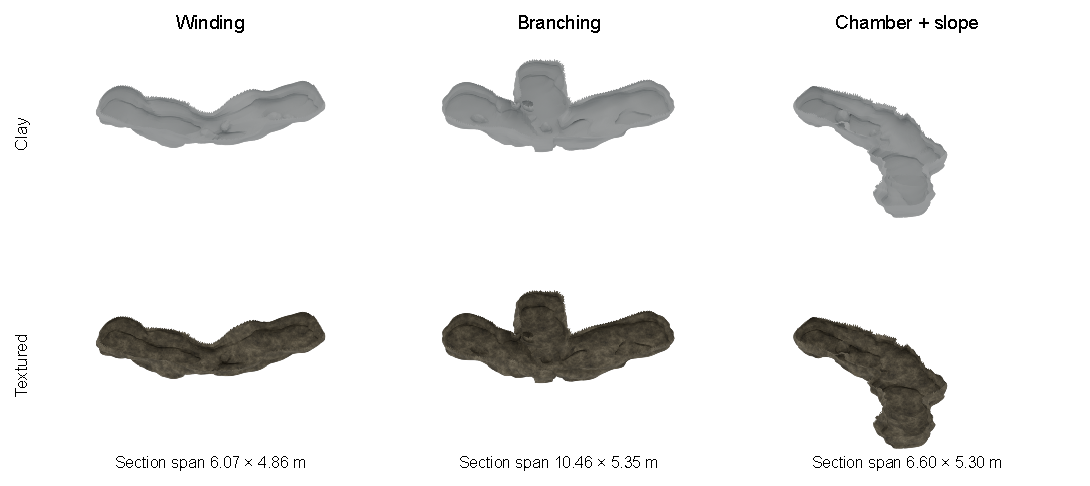
\includegraphics[width=\textwidth]{figures/generated/c1_v02/fixed_cave_cases.pdf}
\caption{Three fixed normal pilot requests, rendered from actual meshes with
the same orthographic scale and view. Clay and textured rows share geometry
and flat normals. Roof removal is an inspection cutaway only. Labels are
mean transverse section spans on delivered visual meshes, including junctions
and chambers; they are not nominal configuration values.}
\label{fig:cases}
\end{figure*}
\begin{figure*}[t]
\centering
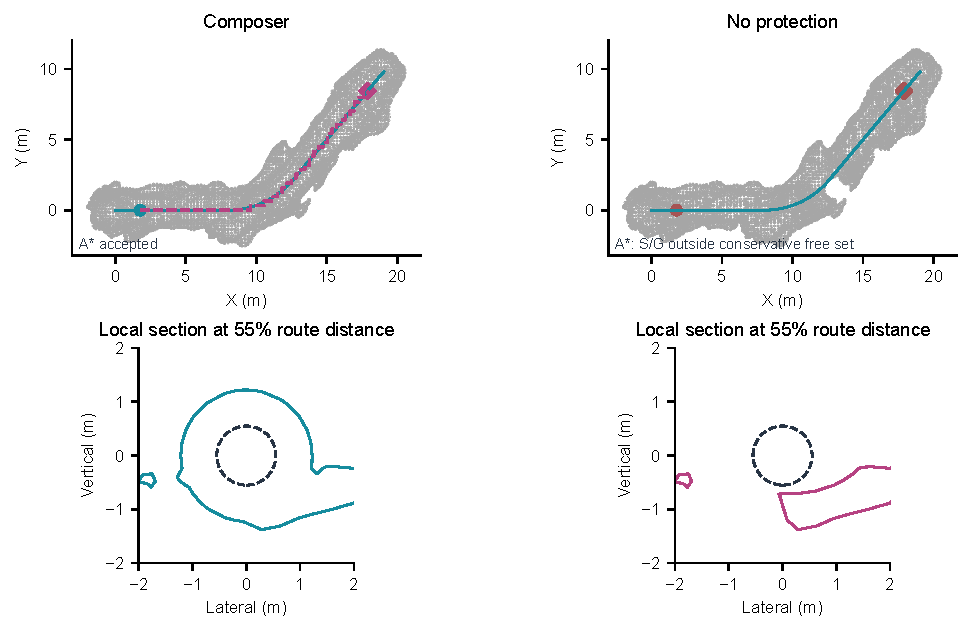
\includegraphics[width=.88\textwidth]{figures/generated/c1_v02/protection_actual_geometry.pdf}
\caption{Fixed stress request with and without passage protection. Gray points
are projections of actual triangle centroids, not a sensed point cloud. Teal
is the construction route; the dashed magenta curve is an independently
searched path, not a robot trajectory. The unprotected mesh is a retained
failed diagnostic: both red endpoint markers fail the conservative-grid gate,
which does not prove continuous-space infeasibility. Matched local sections
at 55\% of the sampled route show geometric change; the dashed circle is the
0.55\,m robot-plus-margin envelope. These sections are distinct from the
endpoint rejection locations.}
\label{fig:protection}
\end{figure*}

\subsection{Effect of training environments}
For each baseline separately, train on restricted caves and full Composer
caves under equal interaction, scene and observation budgets. Fix the
implementation, encoder, memory, vehicle and optimization choices within this
comparison, and report wall time separately from environment interactions.
Use multiple independent training seeds; choose the final count and budget
before launch. A fixed generated validation split selects checkpoints and
hyperparameters. Retention across previously encountered cave families is
evaluated with fixed episodes, without retraining a cave-specific policy.

The new interface pilot contains eight scenes, four per condition: two train,
one development and one generated-ID-test scene per condition. All derivatives
and episodes of a base cave share its split across conditions. Twenty-four
fixed episodes comprise sixteen interior pairs and eight portal full-exit
tasks. The primary paired schedule uses one common interior request and one
exit task per scene; eight auxiliary interior tasks are retained separately.
New seeds define new ID geometry, not automatic OOD.

Nominal geometry, robot size, appearance seed and primary request counts are
matched; realized path clearances still differ between conditions and are
reported per pair. This delivery is therefore an interface pilot, not a fully
clearance-matched causal training comparison. Initial portal export records
retain one boundary-overlap alarm. A uniform 5\,cm terminal-inset revision
passes all eight portable texture/geometry checks. Fresh checks cover internal
paths and ordered entrance/exit witnesses on both changed surfaces. Historical
training snapshots remain separate. No learning curve or policy result is
available (Table~\ref{tab:navigation}).
\begin{table}[t]
\centering
\caption{Planned navigation evaluation matrix. Within each algorithm, hold
training and observation budgets fixed. Dashes mean no policy result exists.}
\label{tab:navigation}
\small
\begin{tabular}{llcc}
\toprule
Baseline & Training caves & Generated & Real-source \\
 & & full exit & local tasks \\
\midrule
FlashSAC & Restricted & \missing & \missing \\
FlashSAC & Composer & \missing & \missing \\
Recurrent PPO & Restricted & \missing & \missing \\
Recurrent PPO & Composer & \missing & \missing \\
\bottomrule
\end{tabular}
\end{table}


\subsection{Frozen-policy transfer on local cave tasks}
Candidate real sources include downloaded scan assets, a team-acquired cave
reconstruction and a reconstruction derived from an external dataset.
The acquisition provenance records AC1/Insight9 and Metashape where reported,
with dates, calibration accuracy and scale left unresolved unless supported
by source records. Local exports are currently uncalibrated open scans.
Underwater simulation on dry-cave geometry is distinct from underwater
acquisition and from executing an embodied robot in the physical cave.

Before policy testing, fix short start--goal segments that cover passage
following, local turns, narrowing or elevation changes. A fragment need not
span the entire cave, but it cannot be selected retrospectively from successful
policy trajectories. Each scheduled episode uses one reset and no manual
correction or dense expert waypoints. The same checkpoint, observation
processing, normalizer and inference rule remain frozen for all assigned
episodes, with no test-time fine-tuning.

All derivatives of one physical cave share a source group, including different
scans, crops, textures and file formats. A source used for materials, geometric
priors, training or generator tuning is ineligible as completely untouched
final OOD. Existing metadata records appearance use for two downloaded cave
groups and development use for the earlier real-data prior. Both newly cropped
reconstructions also have long portions designated for training; actual use
is unconfirmed. Their short portions support within-source spatial holdout,
not an automatic unseen-cave claim. Final source eligibility must be resolved
before transfer can be evaluated.

\subsection{Evaluation metrics and uncertainty}
Record success, collision, out-of-bounds and timeout under a fixed termination
precedence. Keep infrastructure aborts and non-executed episodes explicit.
Define remaining traversable distance by a versioned estimator; Euclidean
goal distance and distance along a witness are not interchangeable with a
free-space shortest path. If the estimator is unavailable for an incomplete
scan, report missing distance with a reason. Preserve trajectories and timing
for audit. Report denominators and source-level results, then aggregate over
training seeds and cave groups without treating correlated episodes as
independent environments. With only a few real sources, show individual-source
outcomes rather than hide variation in an overconfident aggregate.
Eligible test episodes, actual platform settings and training budgets remain
to be frozen. Navigation and transfer effects require the missing policy results.
